\section{问题二建模与求解}

为分析高钾和铅钡两类玻璃的分类规律;对于每个类别选择合适的化学成分对其进行亚类划分得出分类结果,并对分类结果的合理性和敏感性进行分析,做流程图如下: 

\begin{figure}[H] 
	\centering %图片居中
	\includegraphics[width=0.7\textwidth]{12.png} %插入图片,[]中设置图片大小,{}中是图片文件名
	\caption{问题二流程图} %最终文档中希望显示的图片标题
	\label{Fig.main13} %用于文内引用的标签
\end{figure}

\subsection{模型准备}

\subsubsection{数据预处理}

用Pandas读取数据后用isnull函数查找缺失值,发现表中数据有缺失值,用众数来补全数据中的缺失值,再次检验未见异常值。

\subsubsection{特征工程}

要求分别在高钾玻璃和铅钡玻璃的化学成分中选择合适的特征进行亚类分析,聚类分析由于以欧几里得距离为组间、组内判别的衡量,往往对特征的要求极高。
先对原来的14个化学成分指标进行标准化:
再利用方差筛选法来对这几个特征进行过滤筛选,公式为:

\begin{equation}
    \sigma_{j}^{2}=\frac{\sum{{{({{y}_{j}}-\overline{{{y}_{j}}})}^{2}}}}{{{n}_{j}}},j=1,\cdots ,14
\end{equation}

求出第$j$类化学成分的的方差值。为了筛选到最优方差范围,取不同方差值检验化学成分数据通过情况,得到方差通过如下表:

\begin{table}[H]
	\centering
	\begin{tabular}{c c c c c} 
		\toprule[1.5pt]
		方差 & 二氧化硅 & 氧化钠 & \dots & 二氧化硫 \\
		\midrule[1pt]
		$\sigma^2=0$ & 未通过 & 未通过 & \dots & 未通过 \\
		\dots & \dots & \dots & \dots & \dots \\
		$\sigma^2=5$ & 通过 & 未通过 & dots & 未通过 \\
		\dots & \dots & \dots & \dots & \dots \\
		$\sigma^2=10$ & 通过 & 未通过 & \dots & 未通过 \\
		\toprule[1.5pt]
	\end{tabular}
\caption{方差通过情况表}
\end{table}

方差等于10已经能够较充分的分离特征明显的变量,故令数据
\begin{equation}
    {\sigma_j}^2 \leq 10
\end{equation}

利用方差法筛选选出特征明显的变量,用VarianceThreshold函数分别选出高钾类玻璃和铅钡类玻璃化学成分主要特征值,结果如下:

\begin{table}[H]
	\centering
	\begin{tabular}{c c c c c} 
		\toprule[1.5pt]
		高钾类玻璃 & 二氧化硅 & 氧化钾 & 氧化钙 & 氧化铝 \\
		\midrule[1pt]
		铅钡类玻璃 & 二氧化硅 & 氧化钡 & 氧化铅 & 五氧化二磷 \\
		\toprule[1.5pt]
	\end{tabular}
\caption{方差筛选后特征}
\end{table}


\subsection{数据可视化浅析高钾玻璃和铅钡玻璃分类规律}

根据以上得到的数据,本文把14个化学成分作为数值特征与玻璃类型(高钾玻璃和铅钡玻璃)进行多变量数据可视化分析,利用matplotlib库得到数据可视化图如下:

\begin{figure}[H] 
	\centering %图片居中
	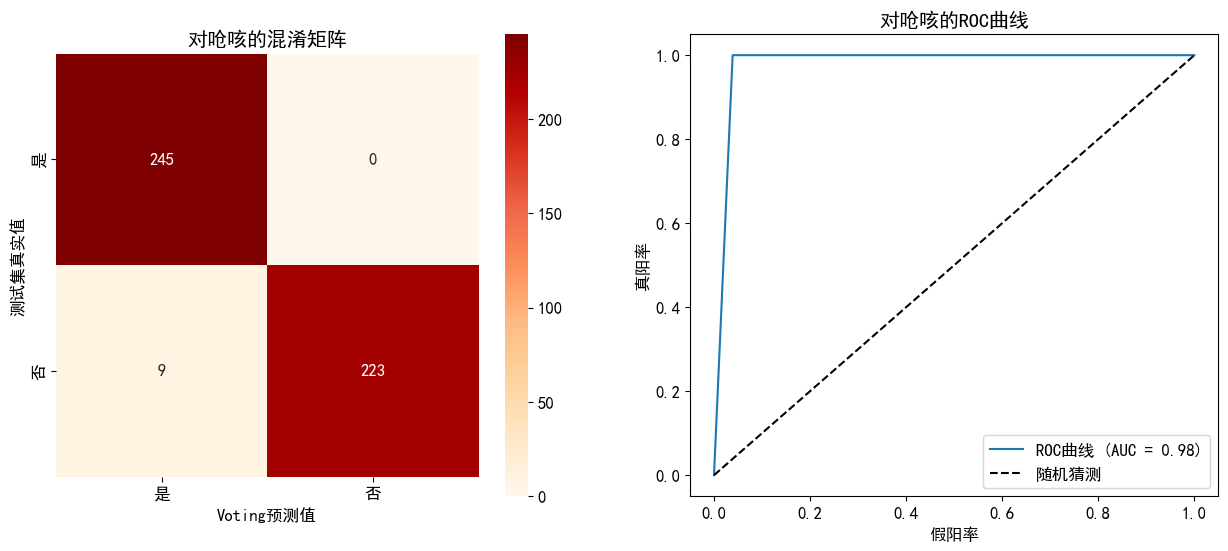
\includegraphics[width=0.7\textwidth]{13.png} %插入图片,[]中设置图片大小,{}中是图片文件名
	\caption{数据可视化图} %最终文档中希望显示的图片标题
	\label{Fig.main14} %用于文内引用的标签
\end{figure}

由图13可知氧化铅、氧化钡、氧化锶、二氧化硫、氧化钾五种化学成分在两种玻璃类型中占比相差极大,其中氧化铅、氧化钡、氧化锶、二氧化硫四种化学成分在高钾类玻璃的含量占比远大于铅钡类玻璃;而氧化钾在高钾类玻璃的含量占比远小于于铅钡类玻璃;氧化钙、氧化锡、氧化铁三种化学成分在高钾类玻璃的含量占比略大于铅钡类玻璃;氧化钠和五氧化二磷两种化学成分在高钾类玻璃的含量占比略于于铅钡类玻璃;而氧化镁、氧化铜两种化学成分在两类玻璃的占比相差不大。

接下来本文分析两个分类特征——纹饰和颜色与玻璃类型之间的关系,分别作多变量分析可视化进行分析,得到数据可视化图如下:

\begin{figure}[H] 
	\centering %图片居中
	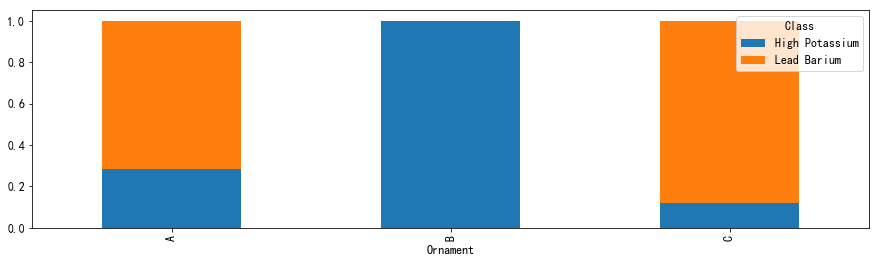
\includegraphics[width=0.7\textwidth]{14.png} %插入图片,[]中设置图片大小,{}中是图片文件名
	\caption{纹饰与玻璃类型可视化图} %最终文档中希望显示的图片标题
	\label{Fig.main15} %用于文内引用的标签
\end{figure}

图14可看出A类纹饰中高钾类玻璃占百分之七十左右,占比大于铅钡类玻璃占比,B类纹饰全是高钾类玻璃,而C类纹饰中高钾类约占百分之九十以上,远大于铅钡类玻璃占比。

\begin{figure}[H] 
	\centering %图片居中
	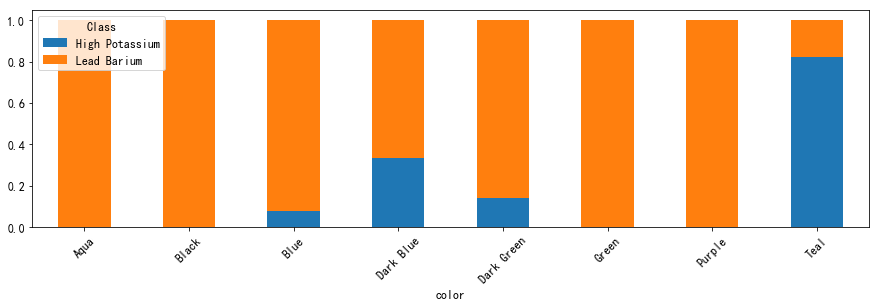
\includegraphics[width=0.7\textwidth]{15.png} %插入图片,[]中设置图片大小,{}中是图片文件名
	\caption{纹饰与玻璃类型可视化图} %最终文档中希望显示的图片标题
	\label{Fig.main16} %用于文内引用的标签
\end{figure}

图15可知浅蓝色样本玻璃中高钾类玻璃占比较大,蓝色、深蓝、深绿三种颜色玻璃中高钾类玻璃占比较小,而其余颜色玻璃中全为铅钡类玻璃。

综上所述,B类纹饰以及蓝绿色、黑色、绿色、紫色的玻璃全为高钾类玻璃;浅蓝色玻璃大部分为高钾玻璃,C类纹饰与蓝色、深绿色玻璃绝大多数多铅钡玻璃。可以得到如下显性分类结果表:

\begin{table}[H]
	\centering
	\begin{tabular}{c c} 
		\toprule[1.5pt]
		高钾玻璃 & B类纹饰、蓝绿色、黑色、绿色、紫色 \\
		\midrule[1pt]
		铅钡玻璃 & C类纹饰、蓝色、深绿色 \\
		\toprule[1.5pt]
	\end{tabular}
\caption{显性分类规律表}
\end{table}

上表可以直观得到两种玻璃的分类标准,下面为了更进一步的分析它们内部分类的本质性规律,决定采用决策树得到内部规律分类。

\subsection{巧用决策树二叉树结构分析两类玻璃分类依据}

决策树是一种经典的传统机器学习分类器,因其独特的树状分类机制,可以让操作者在建模完成后通过调用plot\_tree函数了解每一次树枝分叉的条件,这一特点可以直接达成对玻璃分类依据的探究。

\subsubsection{计算决策树分类结果与本身标签吻合度}

附件早已给出各个样本的玻璃类别,本文通过决策树分类器寻找分类标准,一大前提就是当前决策树的分类结果和玻璃自身标签完全吻合,本文通过混淆矩阵计算决策树分类结果与样本本身标签的吻合度,结果如下:

\begin{figure}[H] 
	\centering %图片居中
	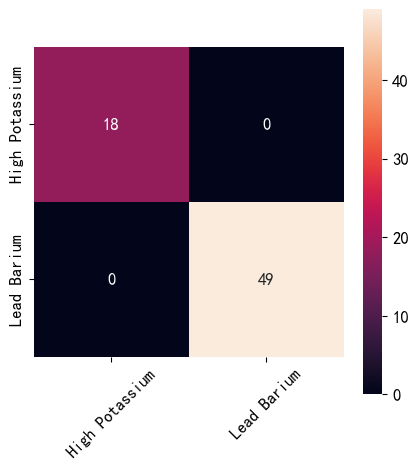
\includegraphics[width=0.7\textwidth]{16.png} %插入图片,[]中设置图片大小,{}中是图片文件名
	\caption{决策树预测结果与样本标签混淆矩阵} %最终文档中希望显示的图片标题
	\label{Fig.main17} %用于文内引用的标签
\end{figure}

由混淆矩阵热力图可知,使用决策树预测的结果与样本自身标签完全匹配。

\subsubsection{决策树的树状结构导出}

通过决策树独特的属性,从sklearn.tree中导入函数plot\_tree作出决策树模型的树状结构,图形如下:

\begin{figure}[H] 
	\centering %图片居中
	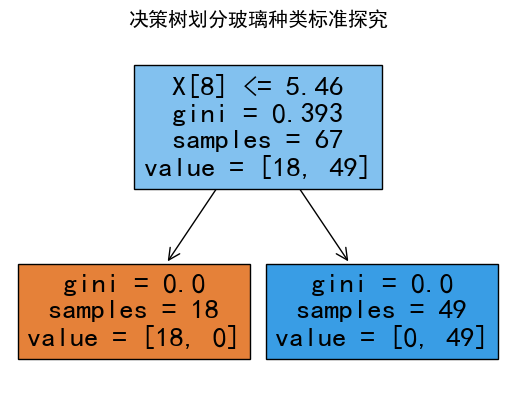
\includegraphics[width=0.7\textwidth]{17.png} %插入图片,[]中设置图片大小,{}中是图片文件名
	\caption{决策树树状结构可视化} %最终文档中希望显示的图片标题
	\label{Fig.main18} %用于文内引用的标签
\end{figure}

通过此图形,本文惊人地发现:决策树所挖掘的数据内在的分类标准与之前看似合理、充分的结果相差甚远——玻璃类比的划分居然只与氧化铅的含量有关!这也进一步告诉本文,简单的数据可视化分析往往只能摸索出浅层次的结论,想要挖掘数据深层次的联系必须通过合适的数据与算法。

\subsection{聚类分析—层次聚类法}

为了对化学成分进行更深层次的分析,又由表8可知每类玻璃分别选出4个变量进行类别划分,利用python中的层次聚类法函数选取三类指标进行划分,分类结果如下表:

\begin{table}[H]
	\centering
	\begin{tabular}{c c c c} 
		\toprule[1.5pt]
		& 第一类 & 第二类 & 第三类 \\
		\midrule[1pt]
		样本编号 & 03,10,12,13,14,18,21,22,27 & 07,09 & 01,04,05,06,15,16,17 \\
		\toprule[1.5pt]
	\end{tabular}
\caption{显性分类规律表}
\end{table}


\begin{table}[H]
	\centering
	\begin{tabular}{c c c c} 
		\toprule[1.5pt]
		& 第一类 & 第二类 & 第三类 \\
		\midrule[1pt]
		样本编号 & 02,19,20,23,32,33,37,39,41,42,43,44,47,48,54,55,56,57,58 & 24,26,30,31,34,35,36,38,40,45,46,49,50,51,52,53	& 08,11,25,28,29 \\ 
		\toprule[1.5pt]
	\end{tabular}
\caption{铅钡类划分结果表}
\end{table}

下面对分类合理性进行检验。

\subsubsection{合理性检验}

本文的目的是为了对分类结果的合理性和敏感性,在对聚类分析结果进行检验时,仅用轮廓系数判断是有失可信度的,CH分数、戴维森堡丁指数(DBI)是对聚类效果评估好坏的评价另外两种方式,下面利用python使用以上三种方法对结果进行检验,得到如下结果:


\begin{table}[H]
	\centering
	\begin{tabular}{c c c c} 
        \toprule[1.5pt]
	    & 轮廓系数 & CH分数 & DBI \\
	    \toprule[1.5pt]
	    高钾玻璃 & 0.448406754 & 36.65655497 & 0.87395307 \\
	    \midrule[1pt]
	    铅钡玻璃 & 0.446694394 & 45.85302210 & 0.82682893 \\
	    \toprule[1.5pt]
	\end{tabular}
\caption{检验结果表}
\end{table}


由上表可知,两类玻璃所得的轮廓系数接近0.5,说明同类样本相距比较接近,聚类效果比较好;CH分数是通过评估类之间方差和类内方差来计算得分,分值越大,表示聚类效果越好,DDB值越小表示聚类结果同簇内部紧密,不同簇分离较远。即类内距离越小,类间距离越大,综上可得出聚类效果较好,该划分方法合理。



\subsubsection{扰动处理}

敏感性分析有很多方法可以实现,依题意所言对结果进行敏感性分析,即探究模型的鲁棒性。本文对被预测标签的数据集进行一定程度的扰动处理,再次预测后通过比较干扰前后的标签差异来衡量模型的稳定性。另外,本文不断对各个特征分别加大干扰,以求探究出影响模型划分类别的“阈值”,用表示高钾玻璃的扰动值,其中表示铅钡玻璃的扰动值,利用公式:

\begin{equation}
    error{{1}_{j}}=\overline{{{y}_{j1}}}*d,d\in \left( 0,+\infty  \right)
\end{equation}

\begin{equation}
    error{{2}_{j}}=\overline{{{y}_{j2}}}*d,d\in \left( 0,+\infty  \right)
\end{equation}

得到每种化学成分的扰动值,带到模型中进行扰动检验,可以得到敏感阈值,最后得出两类玻璃亚类分化的噪音百分比图:

\begin{figure}[H] 
	\centering %图片居中
	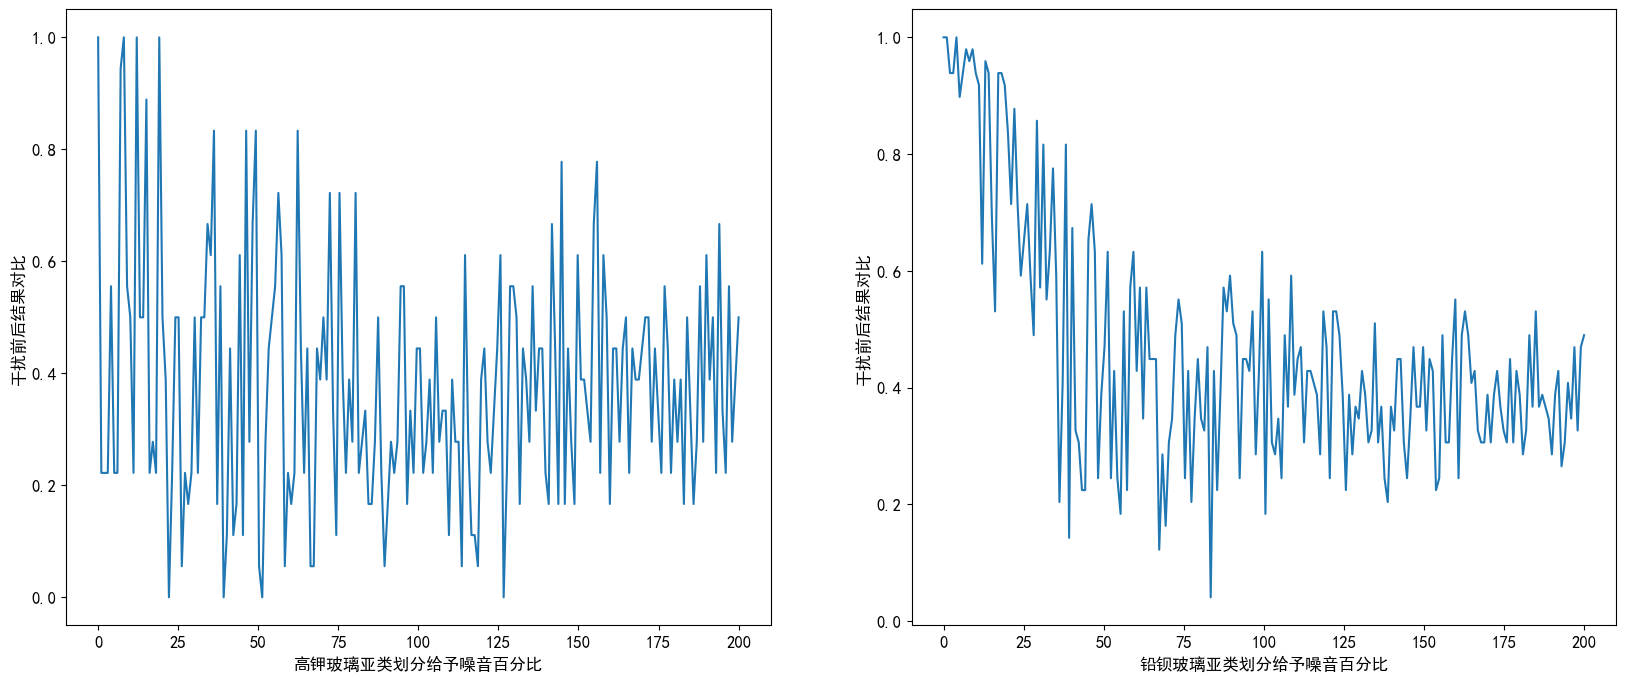
\includegraphics[width=0.7\textwidth]{18.png} %插入图片,[]中设置图片大小,{}中是图片文件名
	\caption{左图为高钾玻璃亚类分化噪音百分比图;右图为铅钡玻璃亚类分化噪音百分比图} %最终文档中希望显示的图片标题
	\label{Fig.main19} %用于文内引用的标签
\end{figure}

通过图18(左)可看出该模型的敏感性阈值d在(0,0.25)之间,模型的准确率都在20\%以上,当d大于0.25时模型的准确率波动性大,预测准确率变化大,因此最好将数据敏感性阈值控制在0.25以内。而对于右图可发现模型的敏感性阈值d在(0,0.1)之间模型的准确率都在90\%以上,当d大于0.10时模型的准确率波动性大,准确率变化大,最好将数据敏感性阈值控制在0.10以内。